% VLDB template version of 2020-03-05 enhances the ACM template, version 1.7.0:
% https://www.acm.org/publications/proceedings-template
% The ACM Latex guide provides further information about the ACM template

\documentclass[sigconf, nonacm]{acmart}

\usepackage{lipsum}

%% The following content must be adapted for the final version
% paper-specific
\newcommand\vldbdoi{XX.XX/XXX.XX}
\newcommand\vldbpages{XXX-XXX}
% issue-specific
\newcommand\vldbvolume{14}
\newcommand\vldbissue{1}
\newcommand\vldbyear{2020}
% should be fine as it is
\newcommand\vldbauthors{\authors}
\newcommand\vldbtitle{\shorttitle} 
% leave empty if no availability url should be set
\newcommand\vldbavailabilityurl{http://vldb.org/pvldb/format_vol14.html}

\begin{document}
\title{A Relational Model of Data for Large Shared Data Banks}

%%
%% The "author" command and its associated commands are used to define the authors and their affiliations.
\author{Ben Trovato}
\affiliation{%
  \institution{Institute for Clarity in Documentation}
  \streetaddress{P.O. Box 1212}
  \city{Dublin}
  \state{Ireland}
  \postcode{43017-6221}
}
\email{trovato@corporation.com}

\author{Lars Th{\o}rv{\"a}ld}
\orcid{0000-0002-1825-0097}
\affiliation{%
  \institution{The Th{\o}rv{\"a}ld Group}
  \streetaddress{1 Th{\o}rv{\"a}ld Circle}
  \city{Hekla}
  \country{Iceland}
}
\email{larst@affiliation.org}

\author{Valerie B\'eranger}
\orcid{0000-0001-5109-3700}
\affiliation{%
  \institution{Inria Paris-Rocquencourt}
  \city{Rocquencourt}
  \country{France}
}
\email{vb@rocquencourt.com}

\author{J\"org von \"Arbach}
\affiliation{%
  \institution{University of T\"ubingen}
  \city{T\"ubingen}
  \country{Germany}
}
\email{jaerbach@uni-tuebingen.edu}
\email{myprivate@email.com}
\email{second@affiliation.mail}

\author{Wang Xiu Ying}
\author{Zhe Zuo}
\affiliation{%
  \institution{East China Normal University}
  \city{Shanghai}
  \country{China}
}
\email{firstname.lastname@ecnu.edu.cn}

\author{Donald Fauntleroy Duck}
\affiliation{%
  \institution{Scientific Writing Academy}
  \city{Duckburg}
  \country{Calisota}
}
\affiliation{%
  \institution{Donald's Second Affiliation}
  \city{City}
  \country{country}
}
\email{donald@swa.edu}

%%
%% The abstract is a short summary of the work to be presented in the
%% article.
\begin{abstract}
Praesent imperdiet, lacus nec varius placerat, est ex eleifend justo, a vulputate leo massa consectetur nunc. Donec posuere in mi ut tempus. Pellentesque sem odio, faucibus non mi in, laoreet maximus arcu. In hac habitasse platea dictumst. Nunc euismod neque eu urna accumsan, vitae vehicula metus tincidunt. Maecenas congue tortor nec varius pellentesque. Pellentesque bibendum libero ac dignissim euismod. Aliquam justo ante, pretium vel mollis sed, consectetur accumsan nibh. Nulla sit amet sollicitudin est. Etiam ullamcorper diam a sapien lacinia faucibus.
\end{abstract}

\maketitle


%%% do not modify the following VLDB block %%
%%% VLDB block start %%%
\begingroup\small\noindent\raggedright\textbf{PVLDB Reference Format:}\\
\vldbauthors. \vldbtitle. PVLDB, \vldbvolume(\vldbissue): \vldbpages, \vldbyear.\\
\href{https://doi.org/\vldbdoi}{doi:\vldbdoi}
\endgroup
\begingroup
\renewcommand\thefootnote{}\footnote{\noindent
This work is licensed under the Creative Commons BY-NC-ND 4.0 International License. Visit \url{https://creativecommons.org/licenses/by-nc-nd/4.0/} to view a copy of this license. For any use beyond those covered by this license, obtain permission by emailing \href{mailto:info@vldb.org}{info@vldb.org}. Copyright is held by the owner/author(s). Publication rights licensed to the VLDB Endowment. \\
\raggedright Proceedings of the VLDB Endowment, Vol. \vldbvolume, No. \vldbissue\ %
ISSN 2150-8097. \\
\href{https://doi.org/\vldbdoi}{doi:\vldbdoi} \\
}\addtocounter{footnote}{-1}\endgroup
%%% VLDB block end %%%

%%% do not modify the following VLDB block %%
%%% VLDB block start %%%
\ifdefempty{\vldbavailabilityurl}{}{
\vspace{.3cm}
\begingroup\small\noindent\raggedright\textbf{PVLDB Availability Tag:}\\
The source code of this research paper has been made publicly available at \url{\vldbavailabilityurl}.
\endgroup
}
%%% VLDB block end %%%

\section{Introduction}

Lorem ipsum dolor sit amet, consectetur adipiscing elit. Suspendisse a arcu quis arcu malesuada ultricies vitae in felis. Curabitur porta lacus at felis viverra hendrerit in non eros. Nam tempus tincidunt metus vitae fermentum. Donec sed risus felis. Cras luctus massa elementum, semper urna vel, efficitur ipsum. Morbi at tellus libero.

Praesent imperdiet, lacus nec varius placerat, est ex eleifend justo, a vulputate leo massa consectetur nunc. Donec posuere in mi ut tempus. Pellentesque sem odio, faucibus non mi in, laoreet maximus arcu. In hac habitasse platea dictumst.Maecenas congue tortor nec varius pellentesque. Etiam ullamcorper diam a sapien lacinia faucibus. Duis vulputate, nisl nec. Donec non odio id neque pharetra ultrices sit amet id purus. Nulla non dictum tellus, id ullamcorper libero. 

\section{Core Structural Elements}

Nulla placerat feugiat augue, id blandit urna pretium nec. Nulla velit sem, tempor vel mauris ut, porta commodo quam. Donec lectus erat, sodales eu mauris eu, fringilla vestibulum nisl. Morbi viverra tellus id lorem faucibus cursus. Quisque et orci in est faucibus semper vel a turpis. Vivamus posuere sed ligula et. 

\subsection{Figures}

Aliquam justo ante, pretium vel mollis sed, consectetur accumsan nibh. Nulla sit amet sollicitudin est. Etiam ullamcorper diam a sapien lacinia faucibus. Duis vulputate, nisl nec tincidunt volutpat, erat orci eleifend diam, eget semper risus est eget nisl. Donec non odio id neque pharetra ultrices sit amet id purus. Nulla non dictum tellus, id ullamcorper libero. Curabitur vitae nulla dapibus, ornare dolor in, efficitur enim. Cras fermentum facilisis elit vitae egestas. Nam vulputate est non tellus efficitur pharetra. Vestibulum ligula est, varius in suscipit vel, porttitor id massa. Nulla placerat feugiat augue, id blandit urna pretium nec. Nulla velit sem, tempor vel mauris ut, porta commodo quam \autoref{fig:duck}.

\begin{figure}
  \centering
  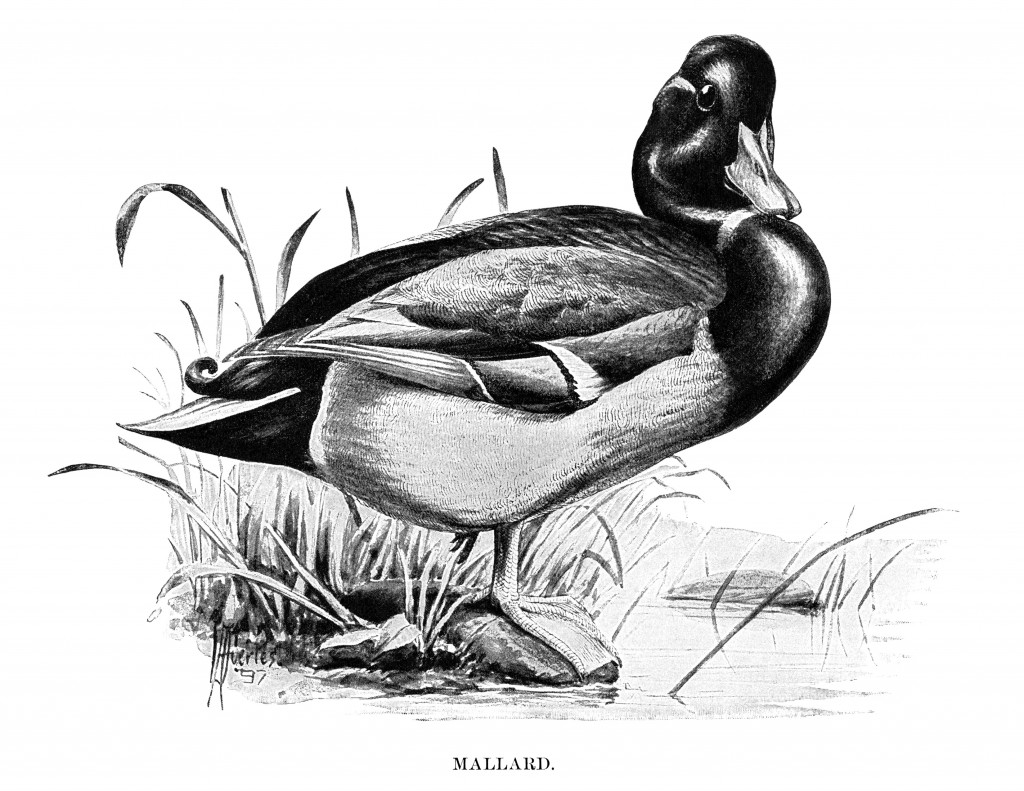
\includegraphics[width=\linewidth]{figures/duck}
  \caption{An illustration of a Mallard Duck. Picture from Mabel Osgood Wright, \textit{Birdcraft}, published 1897.}
  \label{fig:duck}
\end{figure}

\begin{table*}[t]
  \caption{A double column table.}
  \label{tab:commands}
  \begin{tabular}{ccl}
    \toprule
    A Wide Command Column & A Random Number & Comments\\
    \midrule
    \verb|\tabular| & 100& The content of a table \\
    \verb|\table|  & 300 & For floating tables within a single column\\
    \verb|\table*| & 400 & For wider floating tables that span two columns\\
    \bottomrule
  \end{tabular}
\end{table*}

\subsection{Tables}

Curabitur vitae nulla dapibus, ornare dolor in, efficitur enim. Cras fermentum facilisis elit vitae egestas. Mauris porta, neque non rutrum efficitur, odio odio faucibus tortor, vitae imperdiet metus quam vitae eros. Proin porta dictum accumsan \autoref{tab:commands}.

Duis cursus maximus facilisis. Integer euismod, purus et condimentum suscipit, augue turpis euismod libero, ac porttitor tellus neque eu enim. Nam vulputate est non tellus efficitur pharetra. Aenean molestie tristique venenatis. Nam congue pulvinar vehicula. Duis lacinia mollis purus, ac aliquet arcu dignissim ac \autoref{tab:freq}. 

\begin{table}[hb]% h asks to places the floating element [h]ere.
  \caption{Frequency of Special Characters}
  \label{tab:freq}
  \begin{tabular}{ccl}
    \toprule
    Non-English or Math & Frequency & Comments\\
    \midrule
    \O & 1 in 1000& For Swedish names\\
    $\pi$ & 1 in 5 & Common in math\\
    \$ & 4 in 5 & Used in business\\
    $\Psi^2_1$ & 1 in 40\,000 & Unexplained usage\\
  \bottomrule
\end{tabular}
\end{table}

Nulla sit amet enim tortor. Ut non felis lectus. Aenean quis felis faucibus, efficitur magna vitae. Curabitur ut mauris vel augue tempor suscipit eget eget lacus. Sed pulvinar lobortis dictum. Aliquam dapibus a velit.

\subsection{Listings and Styles}

Aenean malesuada fringilla felis, vel hendrerit enim feugiat et. Proin dictum ante nec tortor bibendum viverra. Curabitur non nibh ut mauris egestas ultrices consequat non odio.

\begin{itemize}
\item Duis lacinia mollis purus, ac aliquet arcu dignissim ac. Vivamus accumsan sollicitudin dui, sed porta sem consequat.
\item Curabitur ut mauris vel augue tempor suscipit eget eget lacus. Sed pulvinar lobortis dictum. Aliquam dapibus a velit.
\item Curabitur vitae nulla dapibus, ornare dolor in, efficitur enim.
\end{itemize}

Ut sagittis, massa nec rhoncus dignissim, urna ipsum vestibulum odio, ac dapibus massa lorem a dui. Nulla sit amet enim tortor. Ut non felis lectus. Aenean quis felis faucibus, efficitur magna vitae. 

\begin{enumerate}
\item Duis lacinia mollis purus, ac aliquet arcu dignissim ac. Vivamus accumsan sollicitudin dui, sed porta sem consequat.
\item Curabitur ut mauris vel augue tempor suscipit eget eget lacus. Sed pulvinar lobortis dictum. Aliquam dapibus a velit.
\item Curabitur vitae nulla dapibus, ornare dolor in, efficitur enim.
\end{enumerate}

Cras fermentum facilisis elit vitae egestas. Mauris porta, neque non rutrum efficitur, odio odio faucibus tortor, vitae imperdiet metus quam vitae eros. Proin porta dictum accumsan. Aliquam dapibus a velit. Curabitur vitae nulla dapibus, ornare dolor in, efficitur enim. Ut maximus mi id arcu ultricies feugiat. Phasellus facilisis purus ac ipsum varius bibendum.

\subsection{Math and Equations}

Curabitur vitae nulla dapibus, ornare dolor in, efficitur enim. Cras fermentum facilisis elit vitae egestas. Nam vulputate est non tellus efficitur pharetra. Vestibulum ligula est, varius in suscipit vel, porttitor id massa. Cras facilisis suscipit orci, ac tincidunt erat.
\begin{equation}
  \lim_{n\rightarrow \infty}x=0
\end{equation}

Sed pulvinar lobortis dictum. Aliquam dapibus a velit porttitor ultrices. Ut maximus mi id arcu ultricies feugiat. Phasellus facilisis purus ac ipsum varius bibendum. Aenean a quam at massa efficitur tincidunt facilisis sit amet felis. 
\begin{displaymath}
  \sum_{i=0}^{\infty} x + 1
\end{displaymath}

Suspendisse molestie ultricies tincidunt. Praesent metus ex, tempus quis gravida nec, consequat id arcu. Donec maximus fermentum nulla quis maximus.
\begin{equation}
  \sum_{i=0}^{\infty}x_i=\int_{0}^{\pi+2} f
\end{equation}

Curabitur vitae nulla dapibus, ornare dolor in, efficitur enim. Cras fermentum facilisis elit vitae egestas. Nam vulputate est non tellus efficitur pharetra. Vestibulum ligula est, varius in suscipit vel, porttitor id massa. Cras facilisis suscipit orci, ac tincidunt erat.

\section{Citations}

Some examples of references. A paginated journal article~\cite{Abril07}, an enumerated journal article~\cite{Cohen07}, a reference to an entire issue~\cite{JCohen96}, a monograph (whole book) ~\cite{Kosiur01}, a monograph/whole book in a series (see 2a in spec. document)~\cite{Harel79}, a divisible-book such as an anthology or compilation~\cite{Editor00} followed by the same example, however we only output the series if the volume number is given~\cite{Editor00a} (so Editor00a's series should NOT be present since it has no vol. no.), a chapter in a divisible book~\cite{Spector90}, a chapter in a divisible book in a series~\cite{Douglass98}, a multi-volume work as book~\cite{Knuth97}, an article in a proceedings (of a conference, symposium, workshop for example) (paginated proceedings article)~\cite{Andler79}, a proceedings article with all possible elements~\cite{Smith10}, an example of an enumerated proceedings article~\cite{VanGundy07}, an informally published work~\cite{Harel78}, a doctoral dissertation~\cite{Clarkson85}, a master's thesis~\cite{anisi03}, an finally two online documents or world wide web resources~\cite{Thornburg01, Ablamowicz07}.

%\clearpage

\bibliographystyle{ACM-Reference-Format}
\bibliography{sample}

\end{document}
\endinput
